%%===========================================================%%
%%                                                           %%
%%                       FORWARD PROTONS                     %%
%%                                                           %%
%%===========================================================%%


\chapter{Forward protons}\label{chap:forwardProtons}

The main detector system used in our analyses is the Roman Pot setup in Phase II* configuration (Roman Pots in Phase I took data with STAR during special runs in last days of $p+p$ collisions in 2009, see e.g. Ref.~\cite{A_N,A_N_note,Sikora:2014hca}). It allowed to trigger on forward protons and reconstruct their momentum with high efficiency and precision.

\section{Detector layout}

\begin{figure}[h]\vspace*{-10pt}%
\centering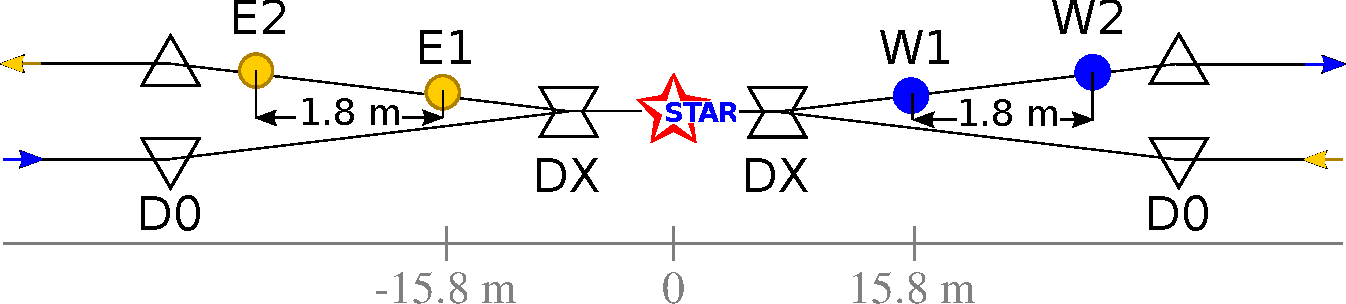
\includegraphics[width=\linewidth]{graphics/rpSim/RP_phaseII.pdf}%
\caption[Schematic represention (top view) of the Roman Pot Phase II* at STAR.]{Schematic represention (top view) of the Roman Pot Phase II* at STAR (not to scale).}\label{fig:RPphaseII}%
\end{figure}

As presented in Figure~\ref{fig:RPphaseII} the Roman Pot Phase II* setup consists of detectors located in two stations on each side of the interaction point (IP) in a distance of 15.8~m and 17.6~m from the IP. Each station has two Roman Pots positioned vertically, one above and the other below the beamline (Fig.~\ref{fig:RpTrackDefinition}). Detectors are situated downstream the DX dipole magnets responsible for head-on targeting of the incoming beams and bending outgoing beams back into the accelerator pipeline. The constant and uniform magnetic field of the DX magnet works as a~spectrometer and thus knowledge on the track angle and position in the detector allows complete reconstruction of the proton momentum, including the fractional momentum loss $\xi$ (as described in~\cite{MomentumReco}). The naming convention of elements of RP setup is described in Ref.~\cite{Labeling}.

Single Roman Pot (the vessel, Fig.~\ref{fig:RPphoto}) houses a package of 4 silicon strip detector planes (Fig.~\ref{fig:SSDphoto}) - one pair of SSDs with vertical and one with horizontal orientation of the strips, and hence measurement of the position of a proton hit is possible in both transverse spatial coordinates, $x$ and $y$. The pitch (distance between neighbouring strips) in a single detector is 100~$\mu$m, therefore intrinsic spatial resolution is at the level of 30~$\mu$m. In addition to the silicon detectors, the package contains plastic scintillator that covers whole active area of the silicon, attached at the back. Two lightguides are glued at the top edge of scintillator which direct the light generated when ionizing particle passes through it to the photomultiplier tubes (PMTs) connected at the very end of each. This counter is used to trigger on forward protons and also provides the timing information.

\section{Roman Pot data reconstruction}

\subsection{Roman Pot track points and tracks}

Roman Pot data is stored in MuDST in StMuRpsCollection. This class contains objects reconstructed with St\_pp2pp\_Maker. The basic (low-level) data objects are the clusters characterized by their length (number of adjacent strips with signal above the threshold), energy (sum of ADC counts in each constituent strip) %
\begin{figure}[hb]%
\centering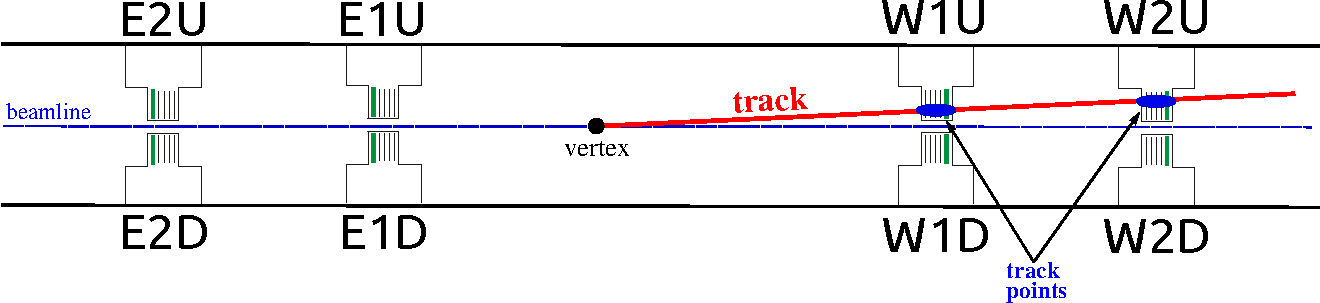
\includegraphics[width=\linewidth]{graphics/rpSim/trackDefinition.pdf}%
\caption[Side view of the Roman Pot Phase II* setup with an illustration of Roman Pot track point and track.]{Side view of the Roman Pot Phase II* setup (not to scale) with an illustration of Roman Pot track point and track.}\label{fig:RpTrackDefinition}%
\end{figure}%
and position. Vectors of clusters are provided independently for each silicon plane. Another low-level data are informations about time (TAC) and signal strength (ADC) for each PMT.

Our physics analyses utilized mainly the high-level objects which are the track points (StMuRpsTrackPoint) and tracks (StMuRpsTrack) stored in vector members of StMuRpsCollection. In short, these objects represent real particles (e.g. their momentum vector) in the same way as the TPC tracks represent particles traversing TPC. Concept of track point and track is depicted in Fig.~\ref{fig:RpTrackDefinition} and  described in some more details in Ref.~\cite{RpInStEvent}.

The algorithm for RP track reconstruction is implemented in St\_pp2pp\_Maker. It is a multi-track algorithm which first forms track points from clusters (there may be many track points in single RP), and then form tracks from all possible combinations of track points in Roman Pots in the same branch~\cite{RpRecoAlgo,RpInStEvent}. The track points and tracks are additionally tuned with Roman Pot ``afterburner'' package (StMuRpsUtil, ~\cite{RpAfterburner}) which recalculates positions of hits and momenta of tracks according to the final alignment corrections and known vertex position.

\subsection{Alignment}

\begin{figure}[b!]%
\centering\vspace{-7pt}%
\parbox{0.495\textwidth}{
  \centering
  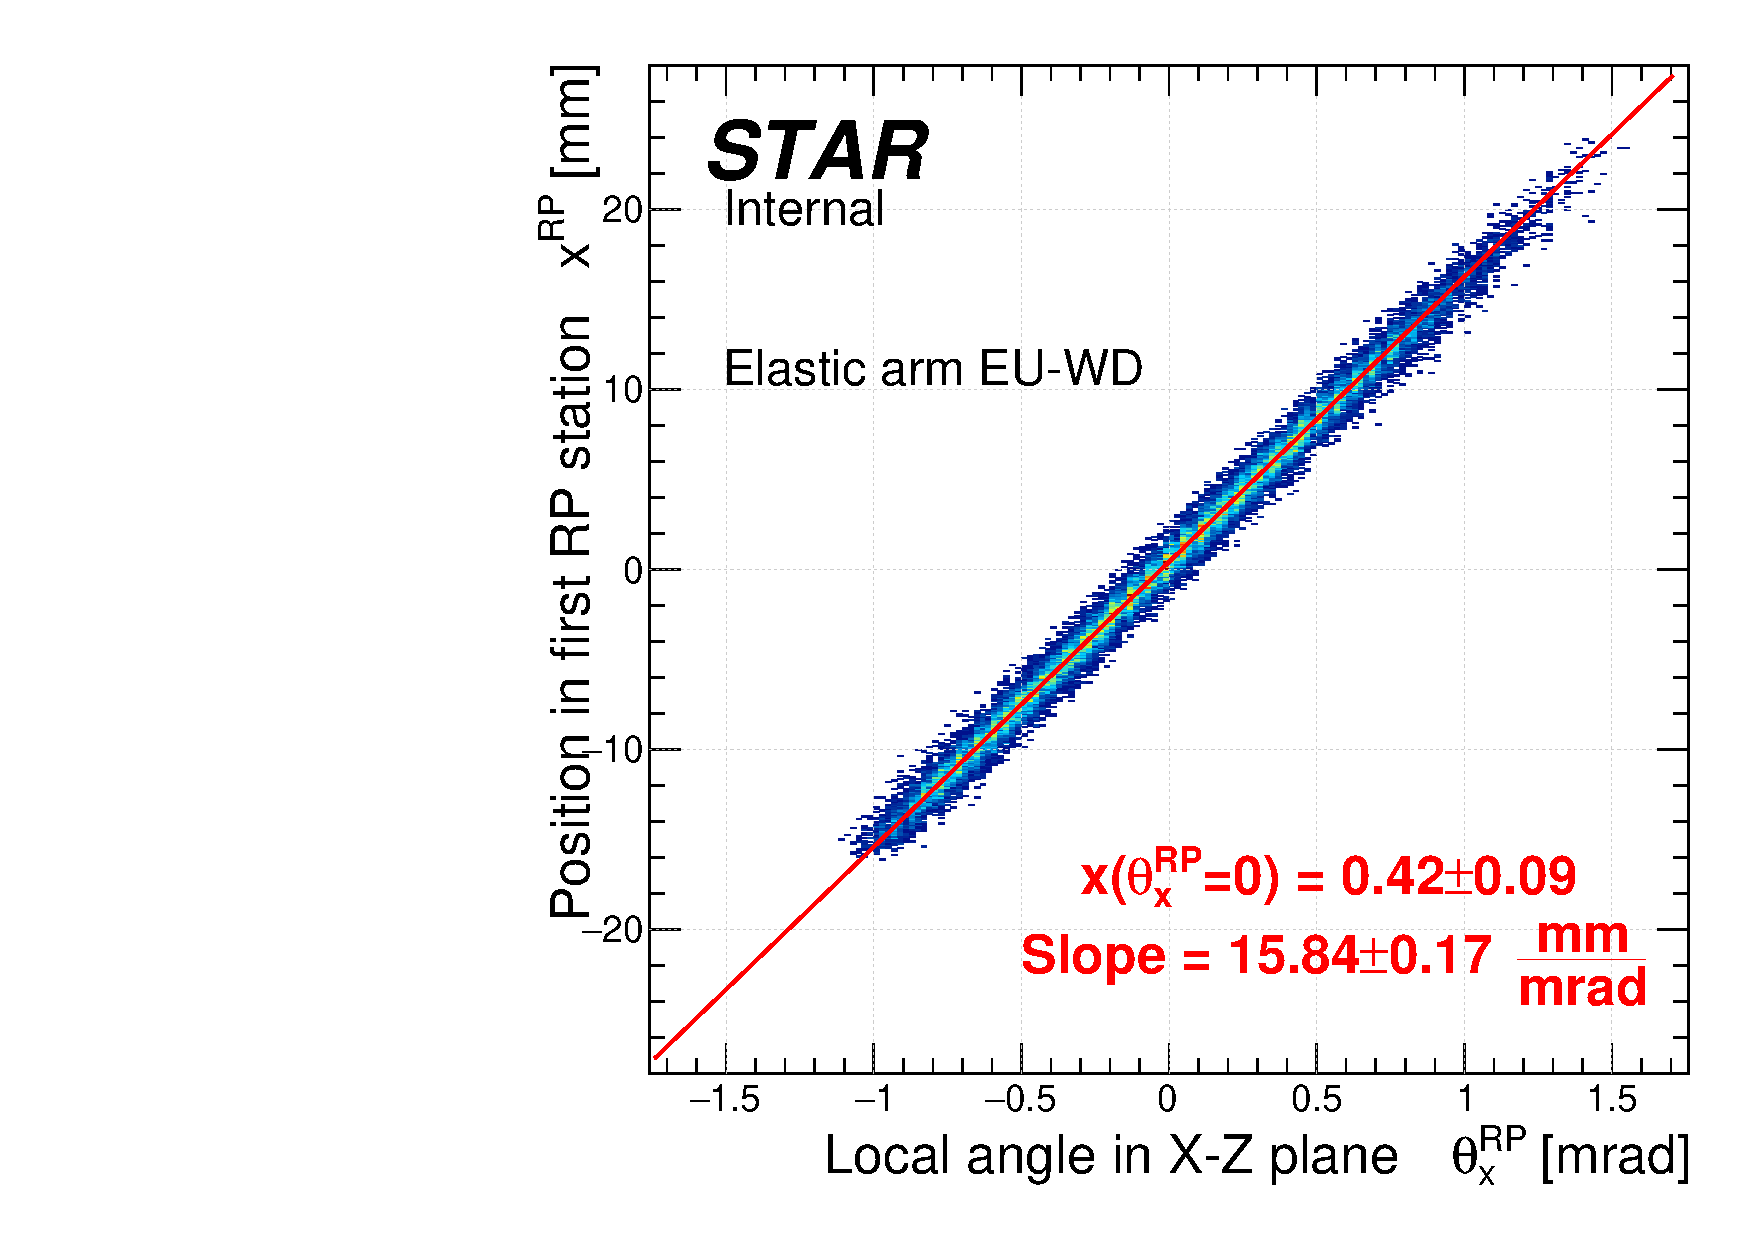
\includegraphics[width=\linewidth,page=1]{graphics/rpSim/VxVy.pdf}\\
  \includegraphics[width=\linewidth,page=2]{graphics/rpSim/VxVy.pdf}
}~
\parbox{0.495\textwidth}{
  \centering
  \includegraphics[width=\linewidth,page=3]{graphics/rpSim/VxVy.pdf}\\
  \includegraphics[width=\linewidth,page=4]{graphics/rpSim/VxVy.pdf}
}\vspace{-5pt}%
\caption[Correlation between the hit position of constituent track point in the first RP station and the local angle of track in elastic scattering events.]%
{Correlation between the hit position of constituent track point in the first RP station ($y$-axis) and the local angle of track ($x$-axis) in elastic scattering events. The $y$-intercept has interpretation of the average position of the interaction vertex in given coordinate.}\label{fig:VxVy}%
\end{figure}


Precise knowledge of positioning of detectors in space is crucial for correct reconstruction of proton momentum. Therefore a process of detector alignment was done, which involved a few steps. At first, dedicated detector survey~\cite{surveyNote} was performed before the start of run 15, which provided initial calibration of the LVDTs installed in Roman Pot movement system. This was sufficient to know the positioning of detectors at a $\gtrsim$1~mm level. Next, the alignment analysis using elastic scattering events was done, as described in the analysis note of elastic proton-proton scattering~\cite{ElasticNote}. This analysis provided detectors alignment at a level of single pitch ($\sim 100\mu\text{m}$). In the last step determination of the average vertex position was done, as described below.

Vertex position is not necessary to correctly reconstruct forward proton observables in elastic scattering events  e.g. squarred four-momentum transfer $|t|$ - this is because one can use momentum balance constraint of elastically scattered protons (collinearity constraint) and calculate scattering angle from the straight line fit to all track points of east and west proton tracks, without knowledge where the interaction vertex was. The same approach cannot be used in other processes like Single or Central Diffraction, since there is only single forward proton (SD) or two forward protons are indepent in terms of scattering angles and momentum loss (CD, CEP).

This fact led to development of the method of extraction of the average vertex position using the elastic scattering data, as presented in Ref.~\cite{AverageVertex}. For this purpose RP\_ET triggers from randomly chosen runs (16085056 and 16085057) were used with single (exactly one) global RP track reconstructed on each side of the IP. Tracks were required to be collinear at 2$\sigma$ level. Selected clean sample of elastic scattering events was used to prepare the plots of the position of the track point in near RP station vs. the local angle of the RP track with respect to the global $z$-axis (Fig.~\ref{fig:VxVy}). The least squares fit of a line (with perpendicular offsets) to all data points in the scatterplot was performed. As a result four lines were obtained, one per arm per transverse coordinate. The slope of the line has interpretation of the distance from the nominal IP ($z=0$) to the $1^{\text{st}}$ RP station at 15.8~m. One can see that the slopes are well consistent with this value. The intercept of the line equals to the average position of the vertex in given coordinate. One finds that $\langle x\rangle_{\text{IP}}$ obtained from the fits to data points in two indepent elastic arms are perfectly consistent, while in $\langle y\rangle_{\text{IP}}$ parameters differ by 1.5 standard deviations. We conclude that extracted values of average positions of the vertex are trustworthy and we can average the numbers obtained from two indepent arms. As a results we use in our analyses numbers $\langle x\rangle_{\text{IP}} = 0.42$~mm, $\langle y\rangle_{\text{IP}} = 0.45$~mm, both in the reconstruction/recalculation of proton tracks with StMuRpsUtil package, and generation of MC events.

In Ref.~\cite{AverageVertex} the method of $\langle z\rangle_{\text{IP}}$ extraction is also presented, however the result $\langle z\rangle_{\text{IP}}= 3$~cm is much smaller than event-by-event variation of the vertex position along $z$-axis (vertex spread is $\sigma(z_{\text{vtx}})=50$~cm), and more importantly it is much less than the distance between nominal IP and the Roman Pots (3~cm compared to 15.8~m). Such small offset has effectively no influence on the error on proton momentum reconstruction, therefore we neglect it.

Due to time dependence of the beam conditions, automatic beam orbit corrections etc., the average position of the vertex may change from run to run. The measure of this variation is a by-product of Roman Pot alignment procedure which was done for every run. In Ref.~\cite{AverageVertexBogdan} the middle points of the track (MPTs, position of the track at $z=0$) are plotted as a function of run number. One can see that MPTs in $x$ and $y$ are roughly constant along the entire data taking period in 2015 and consistent with numbers derived in Fig.~\ref{fig:VxVy}. Another cross-check for the corectness of extracted $\langle x\rangle_{\text{IP}}$ and $\langle y\rangle_{\text{IP}}$ was done with the use of elastic scattering MC simulation in Geant4. Several MC samples were generated with differently positioned vertex. The same procedure was performed as the one described in this section and the output values of $\langle x\rangle_{\text{IP}}$ and $\langle y\rangle_{\text{IP}}$ were always consistent with the true values. Also the comparisons of the hit maps of elastic scattering protons were done between the data and MC, and the best matching was found for vertex generated at $\langle x\rangle_{\text{IP}} = 0.42$~mm and $\langle y\rangle_{\text{IP}} = 0.45$~mm (e.g.~\cite{AlignmentValidation}).


\section{Roman Pot simulation}

\subsection{General description}
Simulation of the STAR detector (STARsim) implemented in Geant3 does not contain a model of the Roman Pot detectors. Because of this, a dedicated simulation program "pp2pp" was prepared to enable precise measurements with the Roman Pot data. The development of this software started in 2012 as two independent projects for ``Geant4 simulation tool kit'' subject at AGH UST, which were later included in B.Sc. theses of the authors. One project was devoted to modeling of the Roman Pot and Silicon Strip Detector package~\cite{BScThesisRafal}, the other was aimed to implement simulation of the collider elements with full magnet lattice (including $B$ field)~\cite{BScThesisLukasz} between the IP and Roman Pot location in Phase I configuration (at $z=\pm55$~m) based on the MAD-X twiss files. At that stage the two programs were used in analyses of 2009 $p+p$ data \cite{MScLukasz,Sikora:2014hca} taken with Roman Pots during special high-$\beta^{*}$ runs. Both projects were merged in 2013 and since then are continuously developed by the Krakow group.

Currently the simulation program is a standalone Geant4 application that allows to simulate any type of particle, track it from the IP to the Roman Pots location (either in Phase I/run 2009 or Phase II*/run 2015\&17 configuration) and obtain the true level and reconstructed information in the standard STAR data format - MuDST classes stored the ROOT tree. In the reconstruction the original STAR St\_pp2pp\_Maker class is used. The program has multiple generation options: the input can be directly from STARsim, Pythia, HepMC format or a simple text file. There are also built-in modes, such as elastic scattering event generation. One can customize the beam conditions, magnet settings (beam energy), Roman Pot positions, and many others. The application is installed at RCF and free to use by any STAR collaborator. Implementation of extensions desired by analyzers is possible after contact with authors. Some more information about the Roman Pot simulation (geometry, usage) can be found in the presentation from the LFS-UPC PWG weekly meeting (Ref.~\cite{Geant4Presentation}).

\subsection{Detector model}

The geometry of the collider elements (beampipe, magnets) and Roman Pot detectors (vessel, SSD packages) is  implemented in Geant4 according to the best available sources of information. The dimensions, positioning and material of the beam pipe and magnets were taken from the technical drawings available at RHIC C-AD and were discussed with the designers of these elements. In case of Roman Pot vessels and detector packages not only technical drawings were used to find the appropriate dimensions, but also dedicated survey was made in which some elements were measured with caliper.

\begin{figure}[h]%
	\vspace{-10pt}\centering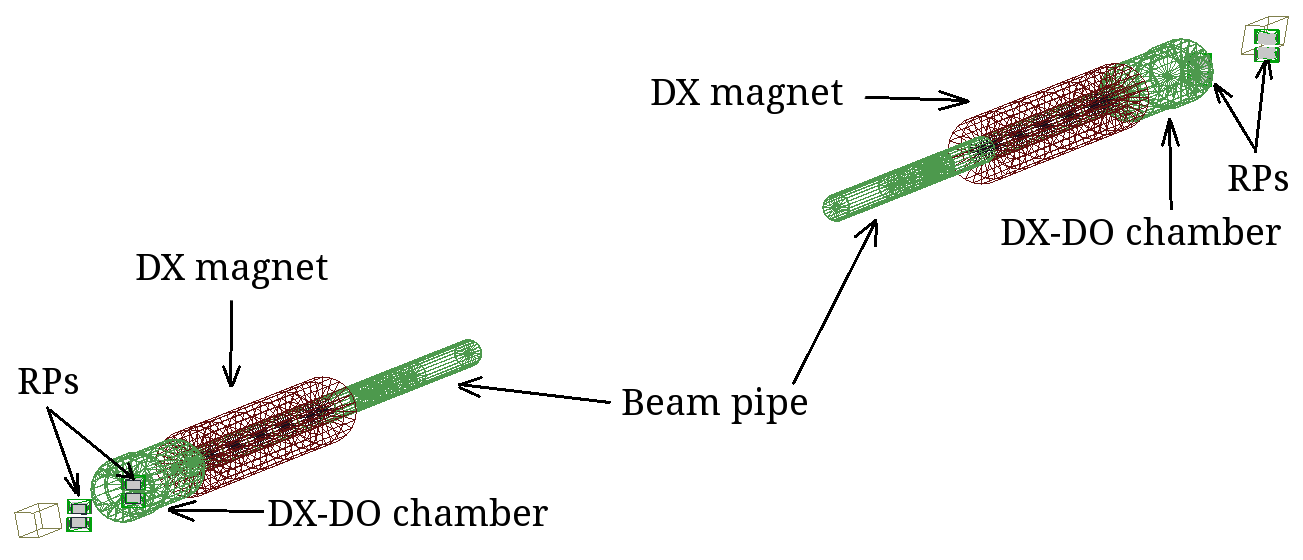
\includegraphics[width=\linewidth]{graphics/rpSim/geant4plot.png}%
	\caption{View of the Geant4 implementation od the Roman Pot Phase II* detector setup.}\label{fig:geant4plot}%
\end{figure}%

In Fig.~\ref{fig:geant4plot} we show the general view of the "world" volume in Geant4 pp2pp simulation with labeled the most significant elements of the geometry. In Fig.~\ref{fig:g4Rp} we show a few shots of the Roman Pot housing and the SSD package implemented in Geant4, together with the real photographs of the Roman Pot and SSD package in Figs.~\ref{fig:RPphoto} and~\ref{fig:SSDphoto}.

%---------------------------
\begin{figure}[h]
	\centering
	\parbox{0.2\textwidth}{
		\centering
		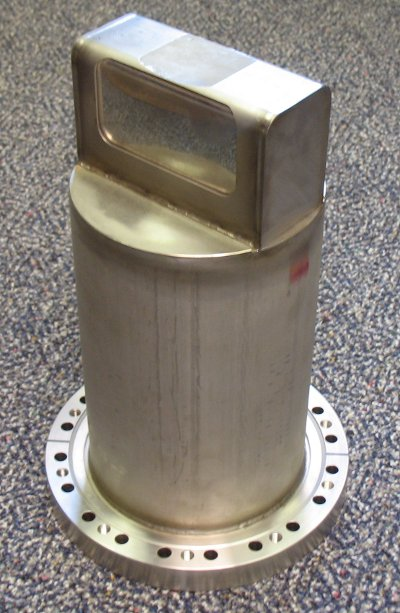
\includegraphics[height=145pt]{graphics/rpSim/romanpot.jpg}
		\caption[Roman Pot vessel (photo).]{Roman Pot vessel (photo).\newline}
		\label{fig:RPphoto}
	}%
	\quad%
	\parbox{0.40\textwidth}{
		\centering
		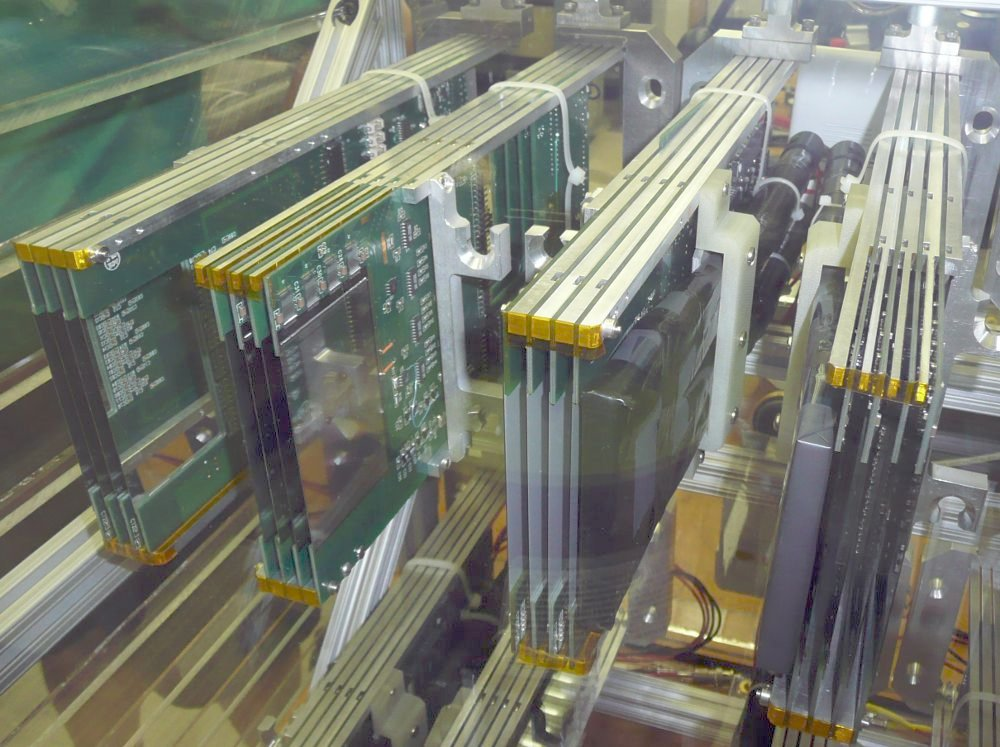
\includegraphics[height=145pt]{graphics/rpSim/SSD.jpg}
		\caption[Silicon Strip Detector packages stored in the protective atmosphere (photo).]{Silicon Strip Detector packages stored in the protective atmosphere (photo).\newline}
		\label{fig:SSDphoto}
	}%
	\quad%
	\parbox{0.33\textwidth}{
		\centering
		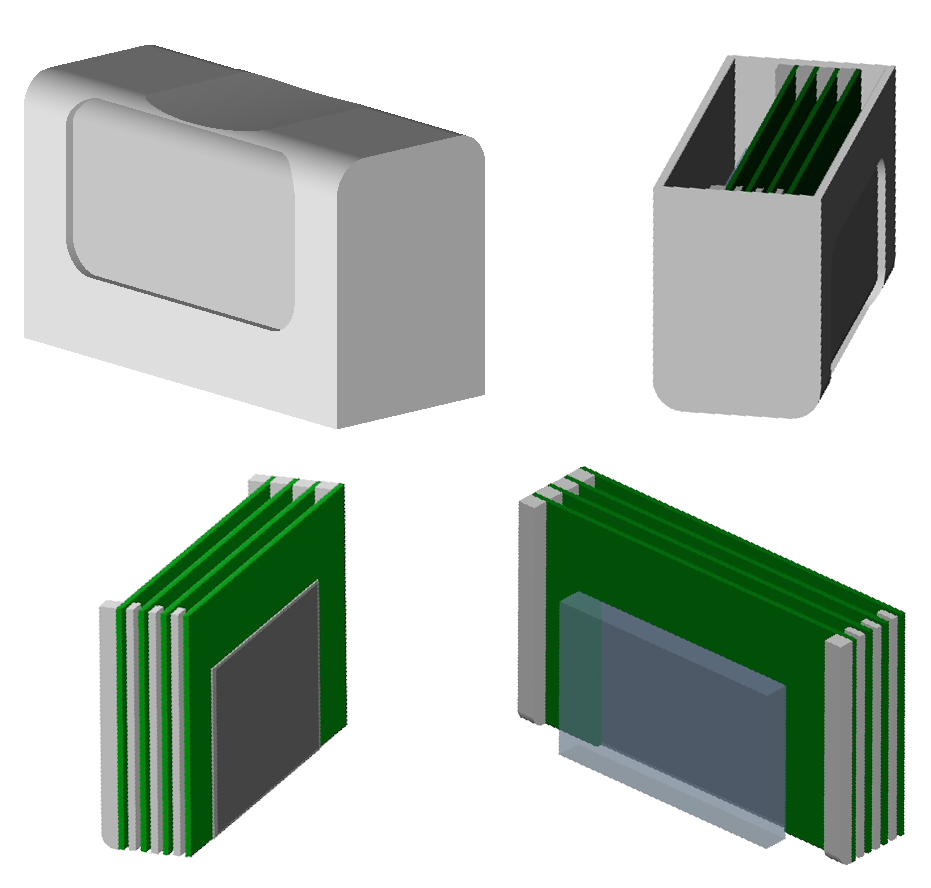
\includegraphics[height=145pt]{graphics/rpSim/g4Rp.png}
		\caption{Geant4 implementations of the Roman Pot vessel and SSD package with trigger counter.}
		\label{fig:g4Rp}
	}
\end{figure}\vspace{-15pt}
%---------------------------

\subsection{Aperture tuning}

It turned out during initial validations of the Geant4 simulation for run 15 with elastic proton-proton scattering events that the distribution of the $(x,y)$ position of the proton in Roman Pots does not agree between the data and MC at a satisfactory level. It was understood that the perfect positioning of the elements of the collider assumed in the geometry model may need some tuning, especially the positioning DX magnet which particularly limits acceptance of the RP detectors. The DX magnets are moved each time the switch between symmetric (e.g. $p+p$) and asymmetric (e.g. $p+Au$) collisions takes place to accommodate for the non-zero tilt of the beams in asymmetric collisions required to close beam orbits and provide collisions in the STAR IR. Therefore lateral offset of this element was expected to be the most significant ingredient needed to correctly describe forward proton acceptance in the RP location.

\begin{figure}[b!]%\vspace{-45pt}
	\centering
	\parbox{0.4725\textwidth}{
		\centering
		\begin{subfigure}[b]{\linewidth}{
				\subcaptionbox{\label{fig:AperturesOnTopOfHitMap_Data}}{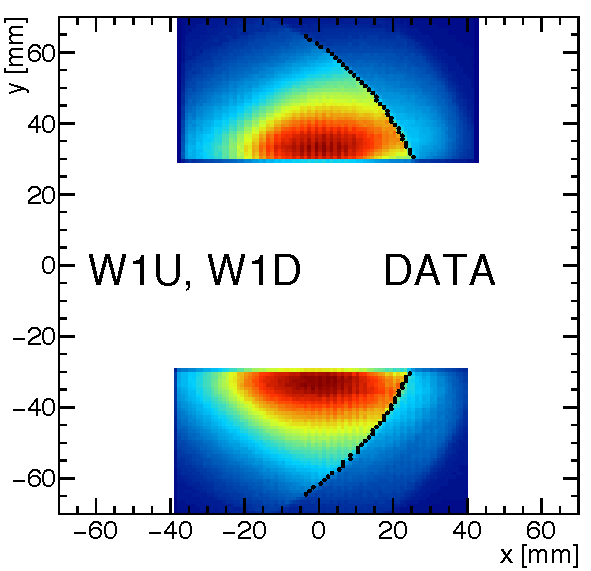
\includegraphics[width=\linewidth]{graphics/rpSim/AperturesOnTopOfHitMap_Data.pdf}\vspace*{-10pt}}}
		\end{subfigure}\\%\\[-3pt]
		\begin{subfigure}[b]{\linewidth}\addtocounter{subfigure}{1}{
				\subcaptionbox{\label{fig:Apertures_swapedAxes_withFit_beforeDxShift}}{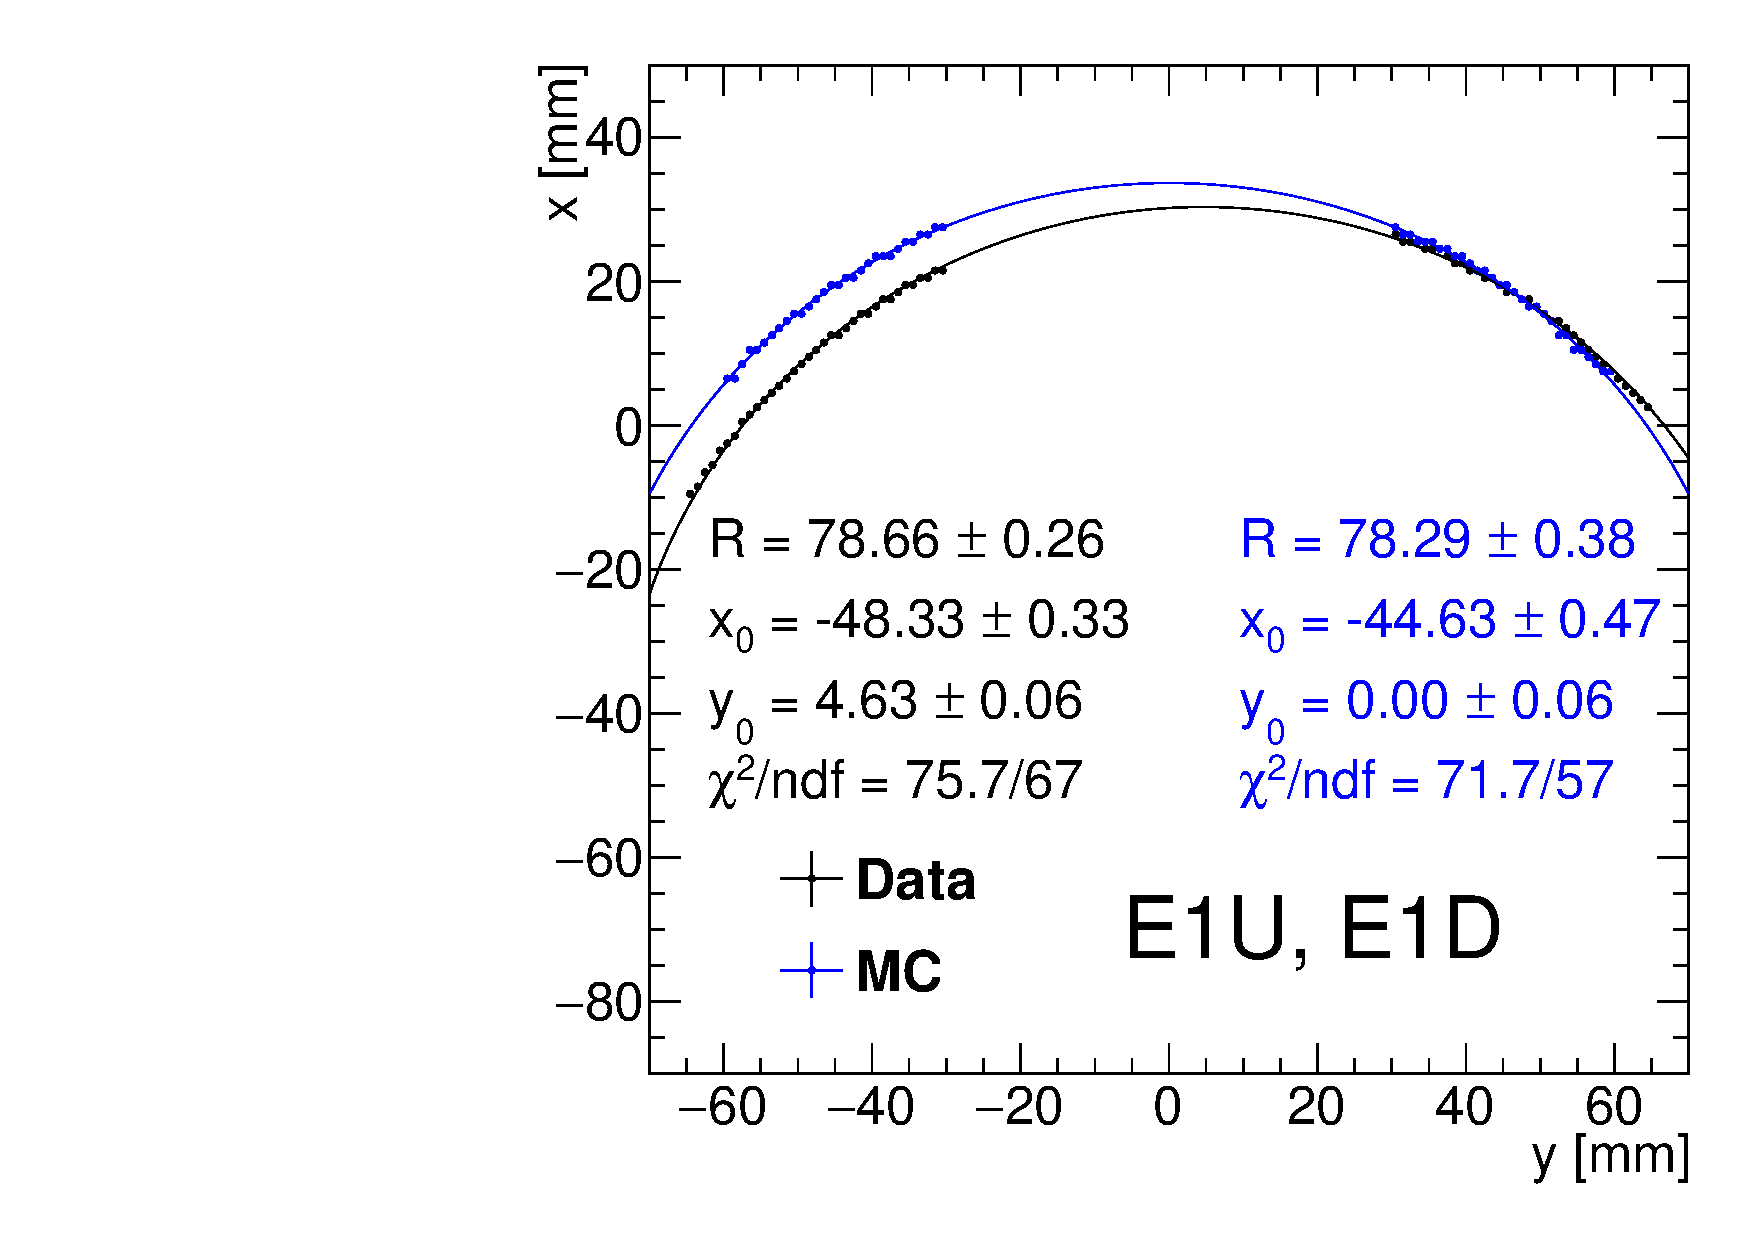
\includegraphics[width=\linewidth]{graphics/rpSim/Apertures_swapedAxes_withFit_beforeDxShift.pdf}\vspace*{-10pt}}}
		\end{subfigure}
	}
	\quad
	\parbox{0.4725\textwidth}{
		\centering
		\begin{subfigure}[b]{\linewidth}\addtocounter{subfigure}{-2}{
				\subcaptionbox{\label{fig:AperturesOnTopOfHitMap_MC}}{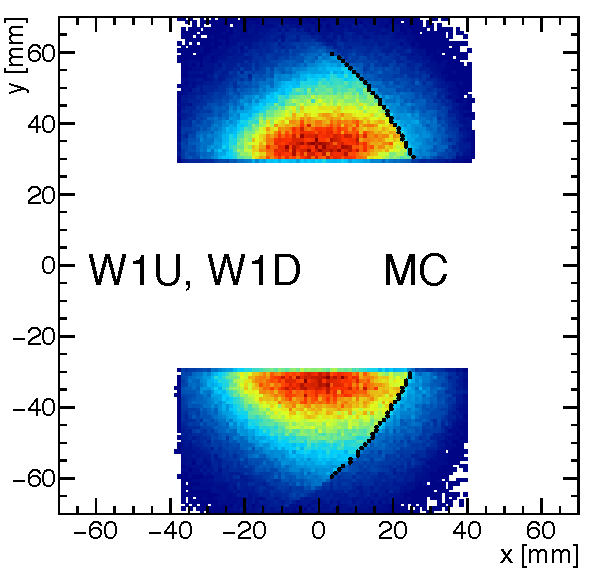
\includegraphics[width=\linewidth]{graphics/rpSim/AperturesOnTopOfHitMap_MC.pdf}\vspace*{-10pt}}}
		\end{subfigure}\\%\\[-3pt]
		\begin{subfigure}[b]{\linewidth}\addtocounter{subfigure}{1}{
				\subcaptionbox{\label{fig:Apertures_swapedAxes_withFit}}{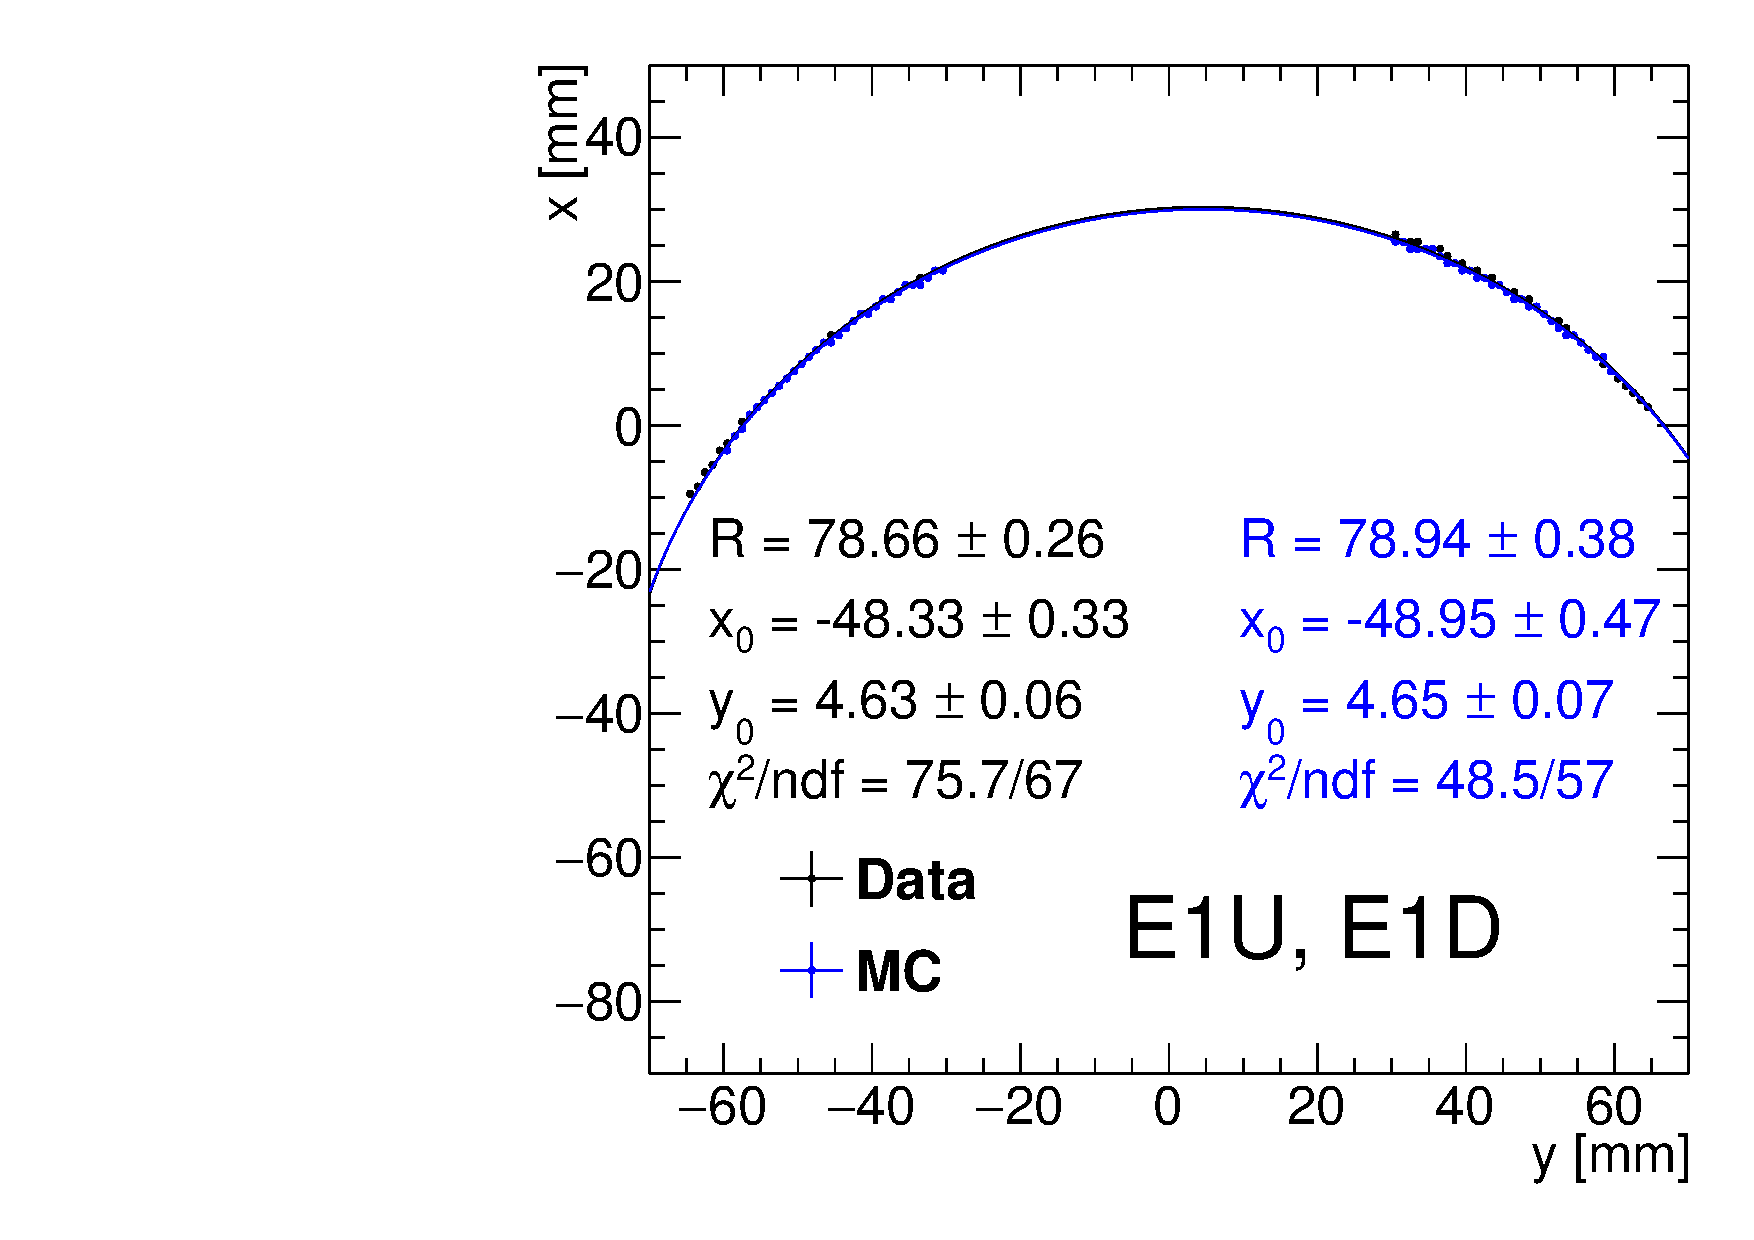
\includegraphics[width=\linewidth]{graphics/rpSim/Apertures_swapedAxes_withFit.pdf}\vspace*{-10pt}}}
		\end{subfigure}
	}%\vspace{-5pt}%
\caption[Sample hit map of elastically scattered protons in the data and MC with extracted envelopes of the DX apertures.]{Sample hit map of track points of proton tracks in events selected as elastic scattering in the data (\ref{fig:AperturesOnTopOfHitMap_Data}) and MC (\ref{fig:AperturesOnTopOfHitMap_MC}) with the DX aperture "shadow" marked with black points. The DX aperture envelopes were fitted with with circles (\ref{fig:Apertures_swapedAxes_withFit_beforeDxShift}) which helped to establish the offsets of DX magnet positions in $x$ and $y$ with respect to the ideal (nominal) geometry, leading to nearly perfect agreement between the data and MC after introducing the offsets in Geant4 geometry (\ref{fig:Apertures_swapedAxes_withFit}).}\label{fig:aperturesWithFit_Sample}%
\end{figure}

In order to quantitatively determine the agreement between the true DX position and position implemented in Geant4 a dedicated analysis of the DX ``shadow'' in the proton hit maps was performed. This algorithm looked for the sharp drop of event counts along the $x$ coordinate in the histogram of $y$- vs. $x$-position of the track points in collinear elastic scattering events with single proton tracks on both sides of the IP. The result (for a single RP station) is presented in Fig.~\ref{fig:AperturesOnTopOfHitMap_Data} and~\ref{fig:AperturesOnTopOfHitMap_MC} for the data and MC, respectively. The envelope of the DX shadow found by the algorithm is marked with black circles. The points were transformed by swapping $x$ and $y$ axis and fitted with a circle, as shown in Fig.~\ref{fig:Apertures_swapedAxes_withFit_beforeDxShift}. The parameters of the circle (radius $R$ and center point $(x_{0}, y_{0})$ ) do not reflect directly the position of the DX, but they were used to find the best shift of the DX on the east and west side in the iterative method. The satisfactory agreement of the DX aperture envelopes between the data and MC was finally found when the shifts of the DX mangnets with respect to their nominal positions were equal to $\Delta x_{\text{DX}}^{\text{East}} = -3.1$~mm, $\Delta y_{\text{DX}}^{\text{East}} = 4.0$~mm, $\Delta x_{\text{DX}}^{\text{West}} = -2.4$~mm, $\Delta y_{\text{DX}}^{\text{West}} = 0.4$~mm. The comparison of the DX shadow envelope after the tune is shown in Fig.~\ref{fig:Apertures_swapedAxes_withFit}. All comparisons are presented in Appendix~\ref{appendix:g4ApertureTuning}.

%\begin{figure}[hb]%
%\caption[Apertures.]{Apertures.}\label{fig:aperturesWithFit_Sample}%
%\centering
%\parbox{0.495\textwidth}{
%  \centering
%  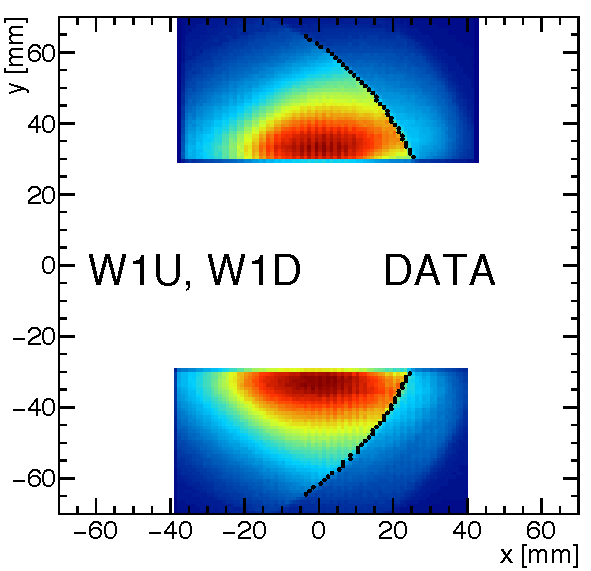
\includegraphics[width=\linewidth,page=1]{graphics/rpSim/AperturesOnTopOfHitMap_Data.pdf}\\
%  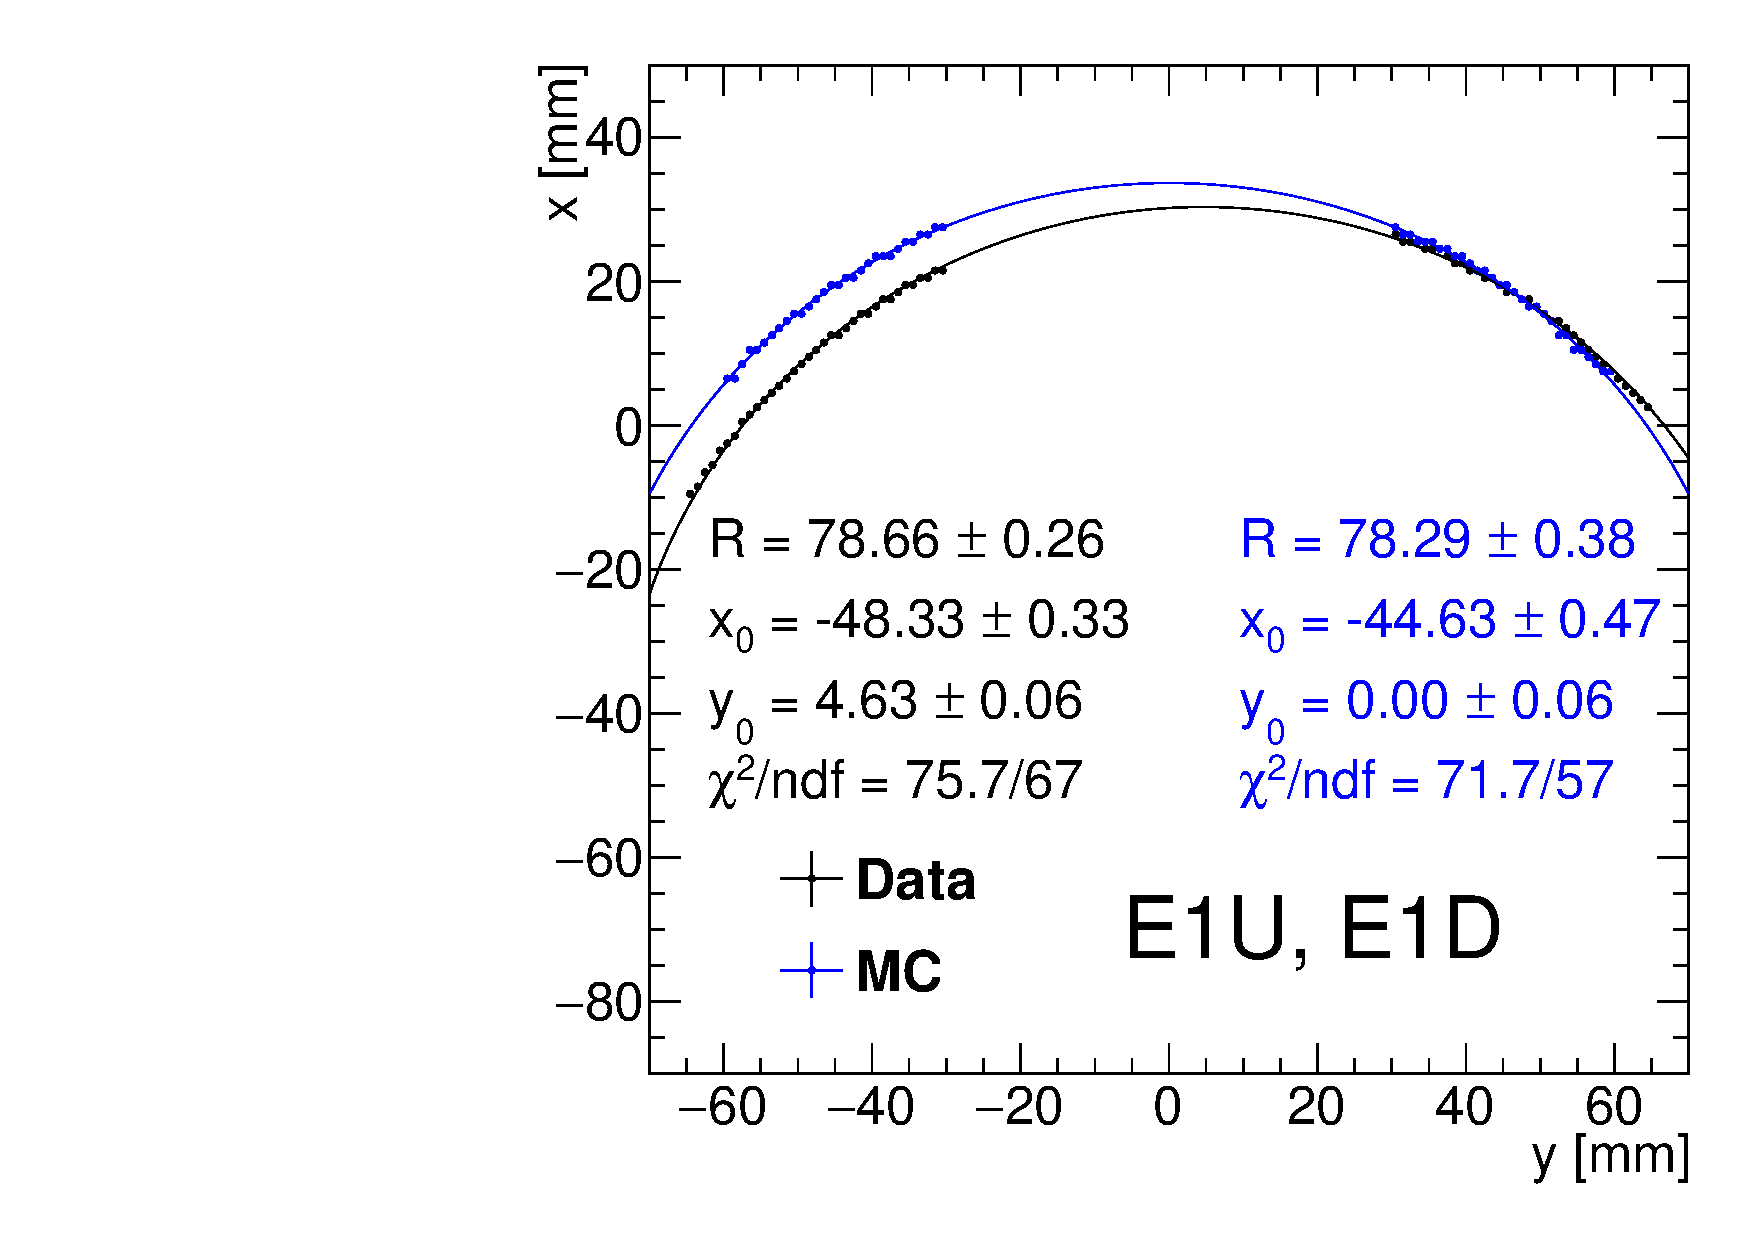
\includegraphics[width=\linewidth,page=1]{graphics/rpSim/Apertures_swapedAxes_withFit_beforeDxShift.pdf}
%}~
%\parbox{0.495\textwidth}{
%  \centering
%  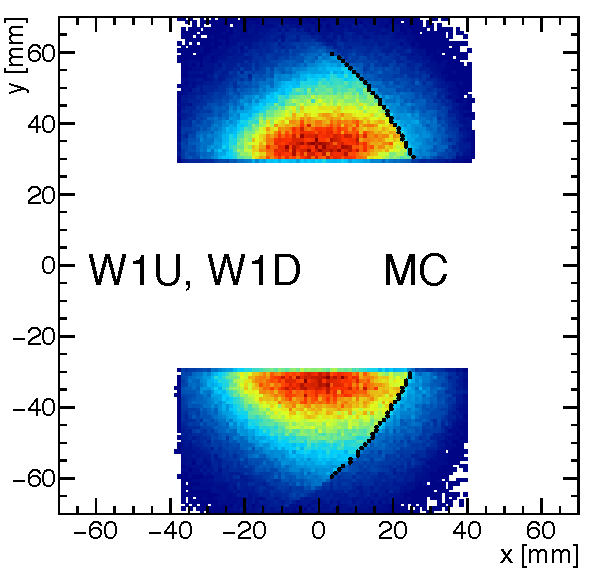
\includegraphics[width=\linewidth,page=1]{graphics/rpSim/AperturesOnTopOfHitMap_MC.pdf}\\
%  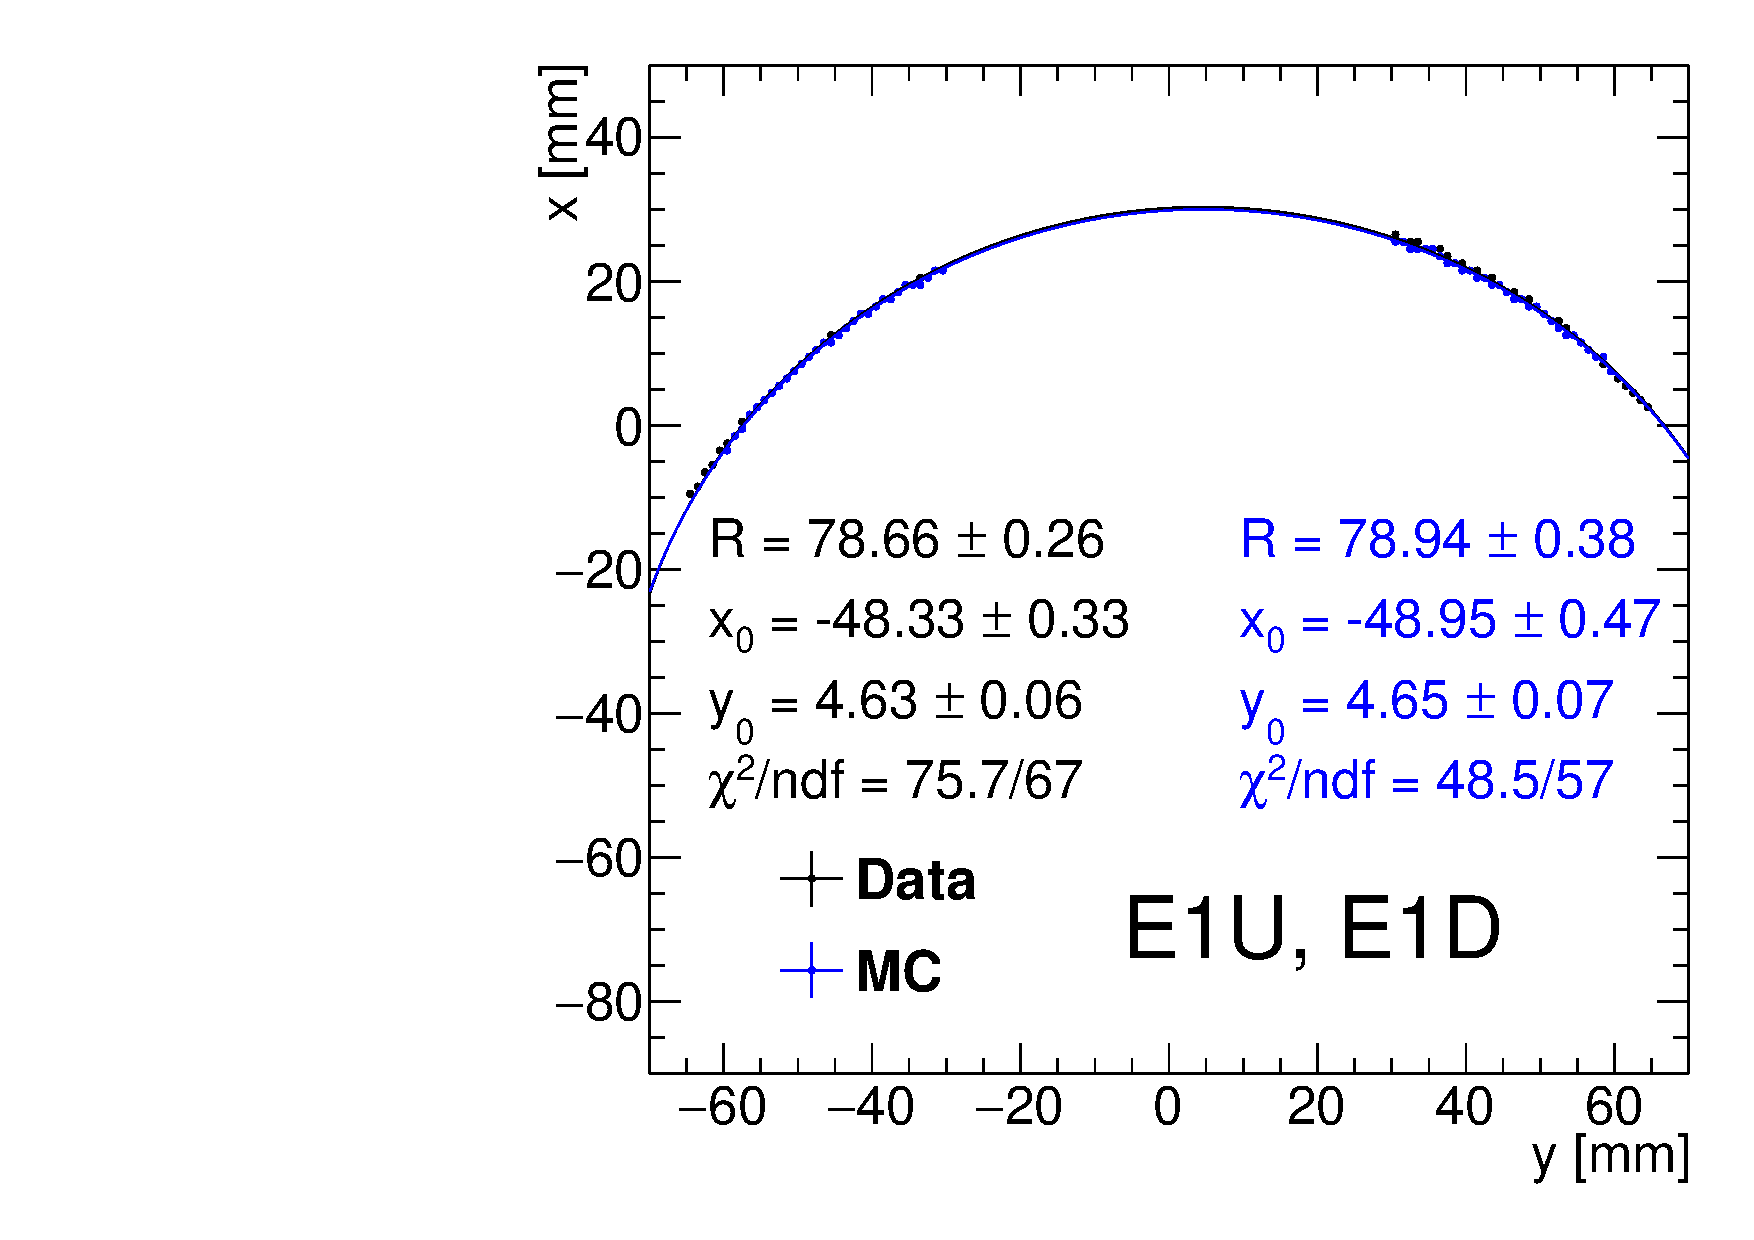
\includegraphics[width=\linewidth,page=1]{graphics/rpSim/Apertures_swapedAxes_withFit.pdf}
%}%
%\end{figure}

\subsection{Embedding technique}

The pp2pp program has an option that allows to overlay the real data with the simulated detector response to MC events. The input data can be any trigger, but most common practice is to embed simulated signal into the zero bias triggers which by definition provide unbiased information about the real environment in which data were collected.

Merging of the simulated signal with the data signal is done for both the SSD data, as well as the PMT data. In case of the PMT data for each channel the ADC (energy) is set to the sum of values in the data and simulation, while the TAC (time) is set to larger value (earlier signal) of the two. In case of the SSD data the merging is done at the level of reconstructed clusters. At the end of simulation of an event a dedicated algorithm is run for every SSD plane which adds vectors of clusters from the data and from the simulation and merges overlapping clusters (recalculates their length, sums energy, updates cluster position). This new collection of clusters is saved in StMuRpsCollection together with new vectors of StMuRpsTrackPoints and StMuRpsTracks reconstructed from this new set of clusters.

The embedding of the RP data has been validated and is used by default in all comparisons of the MC with the data presented in our analysis notes, including this one. The forward proton track reconstruction efficiency obtained from the embedded simulation is consistent with the efficiency estimated from the data within 2\%, as shown in Sec. ADD REF. We consider it a proof for a high quality of the Roman Pot simulation and embedding.